\begin{figure}[ht!]
	\begin{center}
		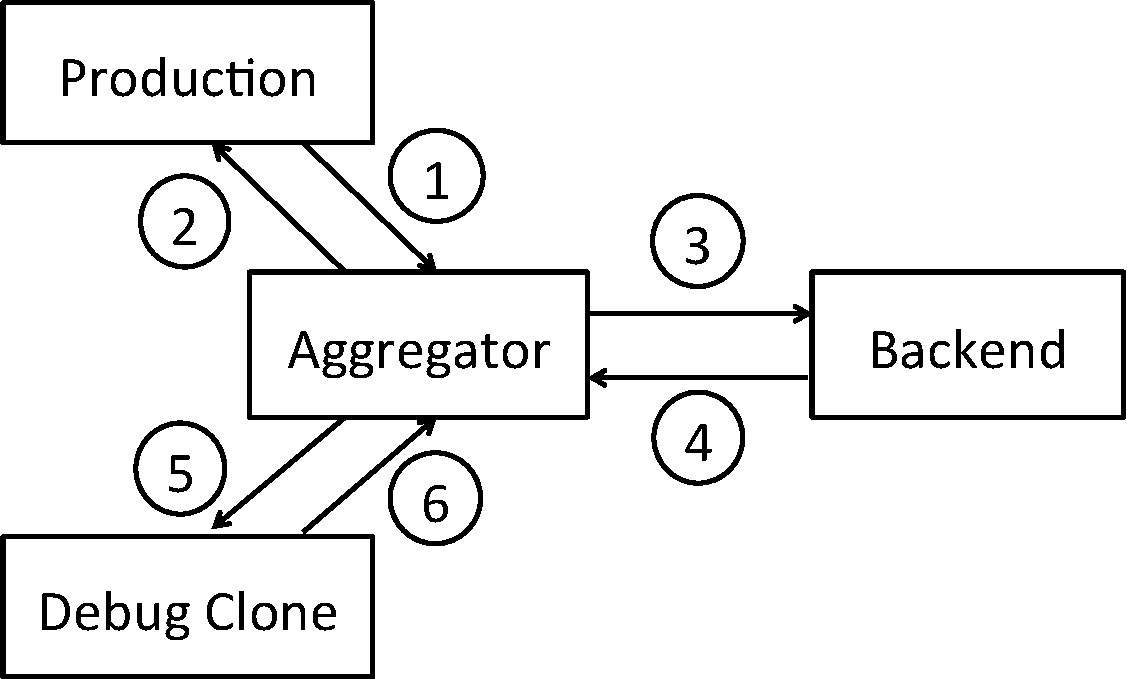
\includegraphics[width=0.4\textwidth]{figs/aggregator.pdf}
		%    \captionsetup{justification=centering}
		\caption{Description of the Network Aggregator. Thread 1 executes step [1,3], Thread 2 step [2,4], and Thread 3 step [5], and Thread 4 step [6]}
		\label{fig:aggregator}
	\end{center}
\end{figure}

\subsection{Proxy Network Aggregator \& Replay }
\label{sec:proxyAggregator}

The proxy described in Section~\ref{sec:proxyDuplicator} is used to forward requests from downstream tiers to production and debug containers.
It manages incoming ``responses'' to the target container, from requests sent to upstream containers.
\xxx{Need to write something that differentiates duplicator and aggregator functionality} 
Imagine if you are trying to debug a mid-tier application container, the proxy network duplicator will replicate all incoming traffic from the client to both debug and the production container. 
Both the debug container and the production, will then try to communicate further to the backend containers.
This means duplicate queries to backend servers (for instance, sending duplicate `delete' messages to MySQL), thereby leading to an inconsistent state.
Nevertheless, to have forward progress the debug-container must be able to communicate and get responses from upstream servers.
The ``proxy aggregator'' module stubs the requests from a duplicate debug container by replaying the responses sent to the production container to the debug-container and dropping all packets sent from it to upstream servers.

As shown in  Figure~\ref{fig:aggregator}, when an incoming request comes to the aggregator, it first checks if the connection is from the production container or debug container. 
In case of the production container (link 1), the aggregator forwards the connection to the backend (link 3). 
Responses from the backend server are sent to the aggregator (link 4), and then forwarded to the production container (link 2) and simultaneously saved in an internal queue.
The aggregator creates an in-memory persistent inter-process FIFO queue for each connection where the responses for each of these connections are stored.
When the corresponding connection from the duplicate debug container connects to the proxy (link 5); all packets being sent are quietly dropped. 
The aggregator then uses the queue to send replies to the debug-container (link 6).
%In a way this is a streaming online record-and-replay, where we are recording the data in our buffer.

We assume that the production and the debug container are in the same state, and are sending the same requests. 
Hence, sending the corresponding responses from the FIFO stack instead of the backend ensures:
(a) all communications to and from the debug container are isolated from the rest of the network,
(b) the debug container gets a logical response for all it's outgoing requests, making forward progress possible,
and (c). similar to the proxy duplicator, the communications from the proxy to internal buffer is non-blocking to ensure no overhead on the production-container.

%In this design we assume that the order of incoming connections remains largely the same.
%To allow for some flexibility, we use a fuzzy checking mechanism using the hash value of the da%ta being sent to correlate the connections. 
%Each queue has a short wait time to check against incoming connections, this allows us to match slightly out of order connections.
%In case a connection cannot be correlated, we send a TCP\_FIN, to close the connection, and inform the user.
%\xxx{Does this come up? Need to talk about that as a limitation if so, or give some evidence that it doesnt otherwise}
%\yyy{you are right removed, actually I needed to update the network aggregator anyways}
%In case a connection cannot be correlated, we allow the connection to time out and send a TCP\_FIN.

